\chapter{Psychological Well-being and Demographic Factors can Mediate Soundscape Pleasantness and Eventfulness}
\label{ch:whostudy}
\markleft{\cref{ch:whostudy}. Psychological Well-being and Demographic Factors}

Soundscape studies aim to consider the holistic human perception of a sound environment, including both the physical phenomena and how these are mediated by internal factors. Within the context of the predictive modelling strategy presented in this thesis, the inclusion of personal factors presents a particular challenge. Referring back to our conceptual model of soundscape perception shown in \cref{fig:percepMap}, the form of the perceptual mapping which translates the soundscape indicators into a listener's perception (expressed via soundscape descriptors) is influenced by the listener's own psychological state and background. Although we can find general patterns in people's responses to soundscape indicators -- for instance, in general people have a strong annoyance reaction to roughness in sirens, but not in horns (see \cref{fig:annoyance-effects}), but this association may not have been formed for everyone equally. Precisely how these responses are formed will differ from person to person. Our next step then, is to investigate to what extent people with similar demographic backgrounds, age, or psychological states share a similar perceptual mapping. In short, we want to determine which personal factors influence the perceptual mapping and how much of the perceptual response can be explained by these factors.

The first step to exploring how we might account for the influence of personal factors is to establish which factors have the most influence and to what extent they can mitigate soundscape perception. Towards this, a first study was conducted on an early subset of the \gls{isd} data, making use of the demographic information (age, gender, educational status, ethnicity, and occupational status) and the psychological well-being included in the \gls{ssid} questionnaire.

% \draft{The initial draft of the text of this study was written by the first author, Mercede Erfanian, based on our joint data collection and statistical modelling performed by me. This study underwent significant revisions following reviewers' comments and the later drafts of the manuscript, particularly the methodology and discussion sections, were written and revised by both Ms Erfanian and myself. Ms Erfanian's focus and expertise is on the psychological aspects of the work, so to maintain consistency with the published version, the background provided on the psychological theory and measures is reproduced verbatim. These sections will be explicitly noted where necessary. is to investigate to what extent the secondary factors mediate soundscape perception and to discuss how they may be incorporated into the predictive soundscape modelling framework.}

\section{Introduction}

Whilst advancements have been made in understanding soundscape determinants, there is a lack of consensus in the literature about the impact of demographic factors on soundscape perception. Additionally, much work in this area relies on limited case studies \citep{Fang2021Soundscape,Ismail2014Sound,Yang2005Soundscape}. There is also a parallel set of literature examining the effect of psychological well-being on sound perception. However, as previous research in this area has typically focused on simple tones rather than complex sounds, controlled laboratory-based experiments, or subsets of individuals \citep{Laufer2016Behavioral,Riskind2014Influence}, the extent to which psychological well-being affects soundscape remains under-researched. Therefore, this study has three aims:

\begin{enumerate}
  \item to determine the associations between soundscape perception and demographic factors (i.e. age, gender, ethnicity, education level, occupation status),
  \item  to understand whether high levels of psychological well-being are associated with increased soundscape pleasantness and eventfulness,
  \item to determine if or how these personal factors should be integrated into a soundscape prediction strategy.
\end{enumerate}

To achieve this we explore the association between personal factors (including psychological well-being and demographics) and the soundscape perception using the \emph{in-situ} data collected in the \gls{isd}. In keeping with the methodology used throughout this thesis, this was investigated through a \gls{mlm}, which incorporates the LocationID as a proxy for contextual information in order to demonstrate what degree of explanatory power these personal factors may have for a predictive model. Finally, I discuss how these results should be considered in the context of my expanded predictive model and what methods may be used to include them as predictors.

\section{Methods}

\subsection{Data collection}
This chapter made use of a subset of data from the \gls{isd}. This study was conducted and published during the first round of \gls{ssid} data collection, prior to the first publication of the ISD. It includes 11 locations in London, with data collected from general members of the public. This chapter made use of the same \gls{ssid} questionnaire presented in full in \cref{app:questionnaire}, which is an adapted version of \citet{ISO12913Part2} Method `A' (urban soundwalk method) and the WHO-5 Well-being Index \citep{Hall2011Examining}, as well as demographic information. As this chapter focusses on the items related to psychological well-being, demographics, and personal factors, we used a subset of the variables available in the full ISD. Only the sections of the questionnaire which were examined within this study are reported in this chapter. \cref{tab:whoDemo} reports the demographic characteristics of the sample used.


\begin{table}[!ht]
  \centering
  \caption{The sample demographic characteristics \label{tab:whoDemo}}
  % \resizebox{\textwidth}{!}{%
  \begin{tabular}{@{}ll@{}}
    \toprule
    Demographic characteristics                 & N(\%)                   \\ \midrule
    Total Samples                               & N = 1134                \\
    \textbf{Gender}                             &                         \\
    \quad Female                                & 610 (53.79)             \\
    \quad Male                                  & 524 (46.2)              \\
    \textbf{Age}                                &                         \\
    \quad Mean                                  & 34.67 years $\pm$ 15.11 \\
    \quad 18-30                                 & 627 (55.29)             \\
    \quad 31-40                                 & 195 (17.19)             \\
    \quad 41-50                                 & 112 (9.87)              \\
    \quad 51-60                                 & 97  (8.55)              \\
    \quad 61-70                                 & 72  (6.34)              \\
    \quad 71+                                   & 31  (2.73)              \\
    \textbf{Educational Level}                  &                         \\
    \quad Some high school                      & 22  (1.2)               \\
    \quad High school graduate                  & 315 (17.3)              \\
    \quad Trade/technical/vocational training   & 51  (2.8)               \\
    \quad University (undergraduate/bachelor)   & 422 (32.1)              \\
    \quad Postgraduate degree (master)          & 324 (17.8)              \\
    \textbf{Occupation Status}                  &                         \\
    \quad Employed                              & 613 (54.05)             \\
    \quad Unemployed                            & 25  (2.2)               \\
    \quad Retired                               & 84  (7.4)               \\
    \quad Student                               & 348 (30.6)              \\
    \quad Employed-Student                      & 5   (0.4)               \\
    \quad Other                                 & 44  (3.8)               \\
    \quad Rather not say                        & 15  (1.3)               \\
    \textbf{Ethnicity}                          &                         \\
    \quad White                                 & 806 (71.08)             \\
    \quad Mixed/Multiple ethnic groups          & 63  (3.5)               \\
    \quad Asian/Asian British                   & 156 (8.6)               \\
    \quad Black/African/Caribbean/Black British & 31  (1.7)               \\
    \quad Middle Eastern                        & 23  (1.3)               \\
    \quad Rather not say                        & 55  (3)                 \\
    \bottomrule
  \end{tabular}%
  % }
\end{table}

\subsubsection*{Psychological well-being/WHO-5 well-being index}
The \glsfirst{who5} is a validated metric used to quantify general well-being. It is measured by asking how individuals have been feeling over the last two weeks through a series of questions such as `I have felt cheerful and in good spirits'. The \gls{who5} has been designed for multiple research and clinical purposes, covering a wide range of mental health domains, namely perinatal mental health, geriatrics mental health, endocrinology, clinical psychometrics, and psychiatric screening.

The \gls{who5} has been shown to be a coherent measure of well-being, with good validity \citep{Topp2015WHO}. For the purpose of analysis, a composite \gls{who5} score is calculated by summing the responses to each of the 5 questions (coded from 0 [for `at no time'] to 5 [for `all of the time']), then multiplying by 4 to get a single score which ranges from 0 (the lowest level of well-being) to 100 (the highest level of well-being) \citep{Topp2015WHO}. \citet{Blom2012Screening} and \citet{LucasCarrasco2012Validity} have confirmed that the \gls{who5} items constitute an integrated scale in which items add up related information about the level of general psychological well-being among both young people and the elderly. 

% \copied{The \glsfirst{who5} asks how individuals have been feeling over the last two weeks such as `I have felt cheerful and in good spirits'. The \gls{who5} has been designed for multiple research and clinical purposes, covering a wide range of mental health domains, namely perinatal mental health, geriatrics mental health, endocrinology, clinical psychometrics, and psychiatric disorders screening.}

% \copied{The \gls{who5} is known to be one of the most valid generic scales for quantification of general well-being. In terms of the construct validity of the scale, \gls{who5} shoed to have properties that are a coherent measure of well-being \citep{Topp2015WHO}. With regards to relevant literature, \gls{who5} confirmed that all items constitute an integrated scale in which items add up related information about the level of general pscyhological well-being among both youngsters and elderlies \citep{Blom2012Screening,LucasCarrasco2012Validity}. For the purpose of analysis, a composite \gls{who5} score is calculated by summing the responses to each of the 5 questions (coded from 0 (for `at no time') to 5 (for `all of the time')), then multiplying by 4 to get a single score which ranges from 0 (the lowest level of well-being) to 100 ( the highest level of well-being) \citep{Topp2015WHO}.}

\subsubsection*{Demographic characteristics}
The demographic characteristics of each participant, including age, gender (male, female, non-conforming), education level (some high school, high school, trade/technical/vocational training, university, postgraduate), occupational status (employed, unemployed, retired, student, employed-student, other, rather not say), and ethnicity (Asian, Black/Caribbean, Middle Eastern, White, Mixed) were collected. Blank spaces were also provided if the participant wished to provide additional information. The demographic breakdown of the sample is presented in \cref{tab:whoDemo}.

\subsubsection*{Outcome variables (\gls{isopl} and \gls{isoev})}
\label{sec:whoOutcomeVar}
The outcome variables used for this study are the \gls{isopl} and \gls{isoev} coordinate values calculated according to Part 3 of \citet{ISO12913Part3}.

% \subsubsection*{Survey procedure}

% The data was collected according to the \gls{ssid} protocol outlined in \cref{chap:protocol}. The goal of the researchers on site was to collect a minimum of one hundred questionnaires from each selected site/location, which was typically achieved over a period of 2-3 days each consisting of approximately a 4 hour session. In some cases, either due to extenuating circumstances, time constraints, or excluded surveys, the full one hundred surveys were not achieved. The data for this chapter were collected from \nth{28} February 2019 to \nth{18} October 2019 between 11 a.m. and 3 p.m.

% In line with the \gls{ssid} protocol, during the survey period, acoustic and environmental metrics were simultaneously collected through binaural recordings, a calibrated \gls{slm}, and an environmental meter which recorded temperature, lighting level, and humidity data. The \gls{slm} was set up in the space in which the questionnaires were conducted (i.e. the \gls{environmental-unit}) and left running for the full duration of the survey in order to characterise the acoustic environment. The environmental metrics were not reported in this chapter since they were not in the scope of this study but are included in \cref{app:location-data} in order to provide context for the interested readers. 

\subsection{Data analysis strategy}

Prior to the data analysis, we imputed missing data and the imputed data was used across all analyses. Missing education values were imputed with the mode value (University). Missing values for age were imputed with the median age value (29). \gls{who5} (psychological well-being) missing values were imputed with the median value (64). We excluded those who responded `non-conforming' (N=4) or `decline' (N=21) for gender, due to the very small sample size and to simplify the effects of gender in the model. The initial data sample size was N=1467; the data included in the analysis N=1134.

\subsubsection*{Correlation between predictors and output variables}
To establish the relationships between all pairs of variables including the predictors and outcome variables, the Pearson correlation coefficient, \gls{anova}, and Chi-square were performed (as appropriate depending on whether the feature was continuous, ordinal, or nominal) between psychological well-being, age, gender, ethnicity, education level, occupation status, and the circumplex coordinate values (\gls{isopl} and \gls{isoev}). These results are given in \cref{tab:whoCorr}.

\subsection{Model specification (linear mixed-effects modelling)}

\glsfirst{lmer} with random intercept and fixed slope, using backward stepwise feature selection was utilised to (a) identify the association of the \glspl{foi} including psychological well-being, age, gender, education level, ethnicity, occupation status, and their interaction terms with \gls{isopl} and \gls{isoev} and (b) accommodate associations within participants among locations. The model is constructed with two levels -- the individual level (the random effects) and the location level (the fixed effects). Separate models were constructed for each \gls{isopl} and \gls{isoev} and take the form:
%
\begin{equation}
  \label{eqn:whoPl}
  ISOPleasant_{ij} = \beta_{0j} + \beta_1 x_{1ij} + \beta_2 x_{2ij} + \ldots + \beta_n x_{nij} + \epsilon_{ij}
\end{equation}
%
\begin{equation}
  \label{eqn:whoEv}
  ISOEventful_{ij} = \beta_{0j} + \beta_1 x_{1ij} + \beta_2 x_{2ij} + \ldots + \beta_n x_{nij} + \epsilon_{ij}
\end{equation}
%
where $ISOPleasant_{ij}$ or $ISOEventful_{ij}$ are the dependent variable value for individual $i$ in Location $j$; $\beta_{0j}$ is the intercept for Location $j$; $\beta_1$ through $\beta_n$ are the slopes relating the independent variables $x_1$ through $x_n$ to the dependent variable; $x_{1ij}$ through $x_{nij}$ are the dependent variables for individual $i$ in Location $j$; $\epsilon_{ij}$ is the random error for individual $i$ in Location $j$. In turn, $\beta_{0j}$ can be expressed as:
%
\begin{equation}
  \beta_{0j} = \gamma_{00} + U_{0j}
\end{equation}
%
where $\gamma_{00}$ is the mean intercept across Locations; and $U_{0j}$ is the unique effect of Location $j$ on the intercept. In a random intercept model, the slope coefficients ($B_n$) are considered fixed across the locations (hence labelled as the fixed effects) indicating that the relationship between the dependent variable (e.g. age, gender, etc.) and the independent variable (\gls{isopl} or \gls{isoev}) is the same for all locations, while the general \gls{isopl} of the location is accounted for by the varying intercept.

In order to identify the significant \glspl{foi} within the multi-level structure, we employed a stepwise feature selection on the fixed effects portion of the mixed-effects model, with an inclusion threshold of $p < 0.05$. Since this model includes only the LocationID at the random effects level, only the fixed effects are reduced in the feature selection process. Once the feature selection process is completed, the final model with only significant \glspl{foi} included is fit and the table of the model coefficients is printed along with plots of the random effects and z-scaled and non-standardised estimates terms.

The model fitting and feature selection was performed using `lme4' (version 1.1) and the `step' function from `lmerTest' (version 3.1.3) \citep{Kuznetsova2017lmerTest} in R statistical software (version 4.0.3) \citep{RCT2018R}. The summaries and plots were created using the `sjPlot' package (version 2.8.6) \citep{Luedecke2021sjPlot}.

\section[Results]{Results\footnote{This section closely resembles the Results section of the original paper \citep{Erfanian2021Psychological} of which I was the second author. I contributed significantly to the drafting of the original paper and in particular to the analysis and results presented here.}}

\subsection{Correlations}

\cref{tab:whoCorr} presents a matrix of the correlation coefficients for the features of interest. It should be noted that these correlations are calculated across the entire pooled sample, and therefore do not account for the multi-level structure of the LocationID. Age, education, gender (male), and \gls{who5} are all positively correlated with \gls{isopl}. However, only age is directly (negatively) correlated with \gls{isoev}. Age, education, and \gls{who5} are all similarly correlated with \gls{isopl}, while gender has a lower effect. It is worth noting that, while occupation is not directly correlated with either of the outcome variables, it is significantly correlated with all of the other independent variables considered in the study and highly correlated with age. As will be noted in the modelling results, this means it can act as a proxy for several of these other features in certain circumstances.

\begin{table}[!h]
  \centering
  \caption{Correlation coefficients for study variables. **$p<0.005$, *$p>0.05$\label{tab:whoCorr}}
  \begin{tabular}{@{}l|lllllll@{}}
    \toprule
    Factors     & Age              & Education       & Ethnicity       & Gender         & Occupation & WHO-5            & ISOPleasant      \\ \midrule
    Age         &                  &                 &                 &                &            &                  &                  \\
    Education   & 0.32             &                 &                 &                &            &                  &                  \\
    Ethnicity   & 0.23             & 0.04            &                 &                &            &                  &                  \\
    Gender      & \textbf{-0.1**}  & 0.05            & \textbf{0.08*}  &                &            &                  &                  \\
    Occupation  & \textbf{0.71**}  & \textbf{0.19**} & \textbf{0.13**} & \textbf{0.1*}  &            &                  &                  \\
    WHO-5       & \textbf{0.12**}  & 0.1             & \textbf{0.1*}   & 0.02           & 0.16       &                  &                  \\
    ISOPleasant & \textbf{0.13**}  & \textbf{0.12**} & 0.11            & \textbf{0.07*} & 0.16       & \textbf{0.14**}  &                  \\
    ISOEventful & \textbf{-0.08**} & 0.08            & 0.07            & 0.05           & 0.12       & 0.00             & \textbf{-0.24**}  \\ \bottomrule
  \end{tabular}
\end{table}

\subsection{Linear mixed-effects modelling}
\label{sec:whoLMERinit}
The linear mixed-effects regression derived regularised models of the soundscape pleasantness and eventfulness. This model was then reduced via backward stepwise feature selection. \cref{tab:whoLMER} presents the \gls{isopl} and \gls{isoev} models, including non-standardised and standardised estimate values and \glspl{ci} for the features that were selected from the initial model. After the feature selection, age, education, and ethnicity were not found to be significant features in either the \gls{isopl} or \gls{isoev} models. It should be noted, however, that the presence of one feature (e.g. occupation) which is highly correlated with another (e.g. age and gender) may cause one of the features to not meet the threshold of significance when both are included, causing it to be removed during the stepwise feature selection. Nonetheless, it may be that, in a final model which included either of these features (but not both), they would each be considered significant. In this way, even though occupation was selected during this process, age may also have been considered significant, when not considering occupation. This behaviour is explored in more detail later.

\begin{table}
\centering
\caption{Fixed and random effects in a linear mixed model explaining variations in \gls{isopl} and \gls{isoev} while controlling for psychological well-being and demographic factors. The standardised estimates are calculated by refitting the model on standardised data scaled by subtracting the mean and dividing by 1 SD, allowing a comparison of all features. **$p<0.005$, *$p>0.05$  \label{tab:whoLMER}}
\resizebox{\linewidth}{!}{%
\begin{tabular}{lccc|ccc} 
\toprule
 & \multicolumn{3}{c|}{\textbf{ISOPleasant}} & \multicolumn{3}{c}{\textbf{ISOEventful}} \\ 
\midrule
\textbf{Predictor} & \textbf{Estimates} & \textbf{Std. Est.} & \textbf{95\% CI} & \textbf{Estimates} & \textbf{Std. Est.} & \textbf{95\% CI} \\
WHO-5 & 0.001** & \textbf{0.03} & 0.01, 0.05 & 0.001 & 0.01 & -0.02, 0.04 \\
Gender (male) & - & - & - & \textbf{-0.08*} & \textbf{-0.04} & -0.07, -0.00 \\
Occupation         (Rather not say) & -0.19* & \textbf{-0.19} & -0.36, -0.02 & \textbf{0.7**} & \textbf{0.02} & -0.13, 0.17 \\
Occupation         (Retired) & 0.1** & 0.10 & 0.03, 0.18 & \textbf{-0.18**} & \textbf{-0.11} & -0.18, -0.04 \\
Occupation         (Unemployed) & 0.01 & 0.01 & -0.13, 0.14 & \textbf{0.01**} & \textbf{0.18} & 0.06, 0.3 \\
WHO-5 x Gender         (male) & - & - & - & \textbf{-0.001*} & \textbf{-0.04} & -0.07, -0.00 \\
WHO-5 x Occupation         (Rather not say) & - & - & - & \textbf{-0.01**} & \textbf{-0.21} & -0.33, -0.09 \\ 
\midrule
\multicolumn{7}{l}{\textbf{Random Effects}} \\ 
\midrule
$\sigma^2$ & \multicolumn{3}{l|}{0.11} & \multicolumn{3}{l}{0.08} \\
$\tau_00$ & \multicolumn{3}{l|}{0.06$_{Location}$} & \multicolumn{3}{l}{0.01$_{Location}$} \\
ICC & \multicolumn{3}{l|}{0.35} & \multicolumn{3}{l}{0.15} \\
N & \multicolumn{3}{l|}{11} & \multicolumn{3}{l}{11} \\ 
\midrule
Observations & \multicolumn{3}{l|}{1134} & \multicolumn{3}{l}{1134} \\
Marginal $R^2$/ Conditional $R^2$ & \multicolumn{3}{l|}{0.014 / 0.354} & \multicolumn{3}{l}{0.039 / 0.181} \\
AIC & \multicolumn{3}{l|}{779.125} & \multicolumn{3}{l}{451.351} \\
\bottomrule
\end{tabular}
}
\end{table}

\subsubsection*{Psychological well-being and its association with pleasantness and eventfulness}

The final models found that a higher level of psychological well-being and retirement are associated with higher pleasantness, while individuals that prefer not to report their occupational status showed a negative association with pleasantness. Further analysis revealed that psychological well-being was negatively associated with eventfulness in men and individuals that did not report their occupational status. Additionally, we detected that eventfulness is positively associated with unemployment, whereas it is negatively associated with gender (male) and retirement (\cref{tab:whoLMER}). 

The marginal and conditional $R^2$ values are given for each model in \cref{tab:whoLMER}. In a mixed effects model, the marginal $R^2$ represents the variance explained by the fixed effects (the individual-level independent variables) while the conditional $R^2$ represents the variance explained by both the fixed and random effects \citep{Nakagawa2012general}. From the conditional $R^2$, we can say that the full models explain 35.4\% and 18.1\% of the variance in \gls{isopl} and \gls{isoev}, respectively (\cref{fig:whoRand}). While the majority of the variance is explained by location-level differences (as confirmed by the \glspl{icc}), 1.4\% of variance in \gls{isopl} and 3.9\% of variance in \gls{isoev} is explained by the \glspl{foi} (i.e. psychological well-being and age) included as fixed effects. It should be noted that the $R^2$ values reported here are lower than the results given in \cref{ch:lockdown}. There are two reasons for this: given the nature of this study, it was not appropriate to summarise the performance of the models in terms of their performance at predicting the average perception of each location, as in \cref{ch:lockdown}. In both cases, the accuracy when attempting to predict the response of each individual is much lower than when the goal is to predict the general perception of a location. The second reason is that this model is focussed on the potential for demographic and personal features to predict soundscape perception. As these results demonstrate, these factors, while they do impact perception and are statistically significant, are much less important for prediction accuracy than the psychoacoustic features included in \cref{ch:lockdown}.

\begin{figure}[!h]
  \centering

  \begin{subfigure}{.75\textwidth}
    \centering
    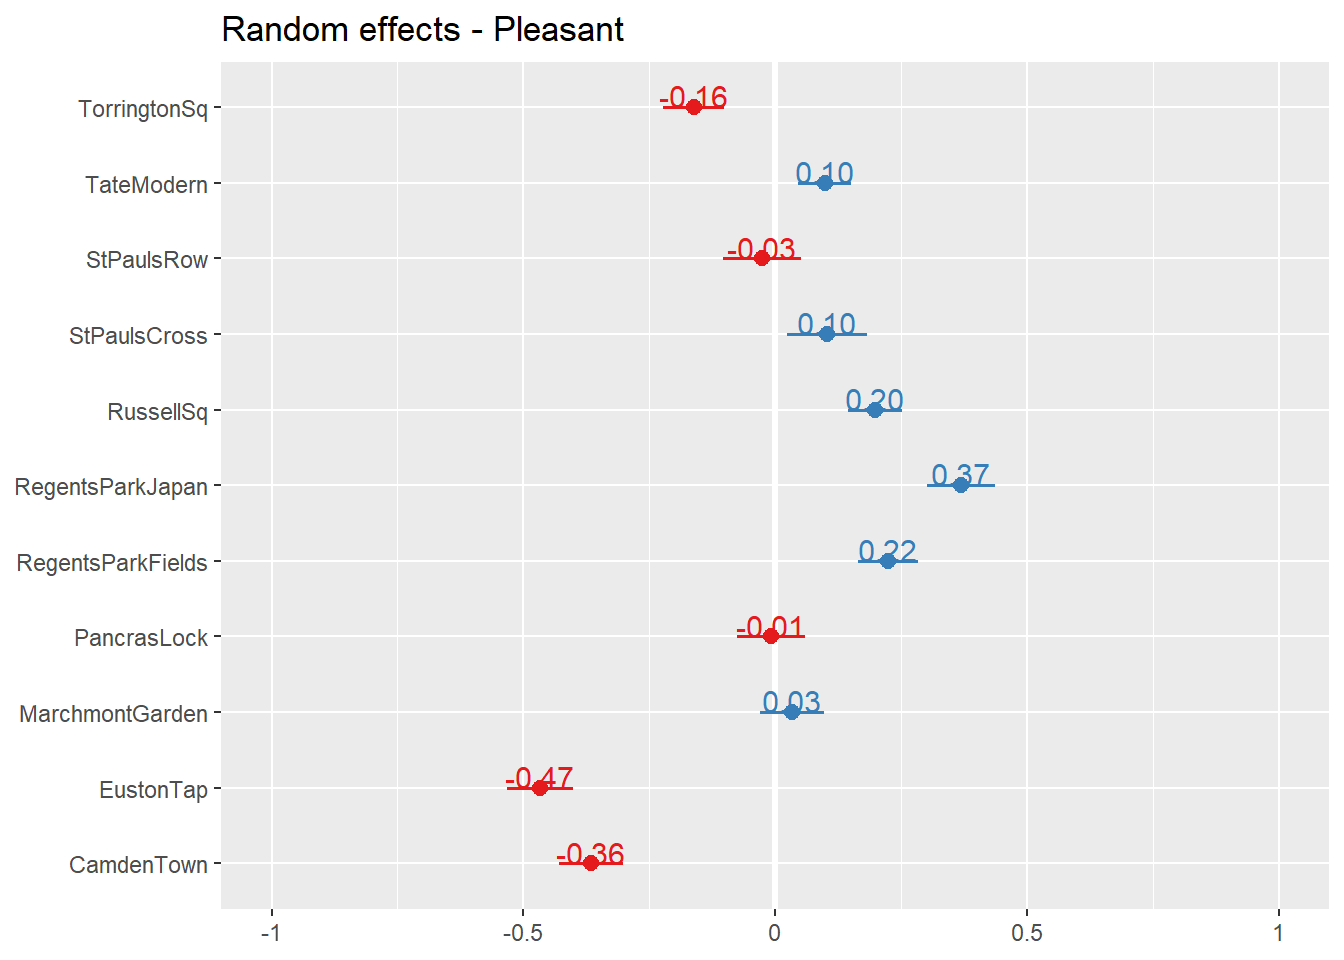
\includegraphics[width=\textwidth]{Figures/whoRandPlNew.png}
  \end{subfigure}%
  \hfill
  \begin{subfigure}{.75\textwidth}
    \centering
    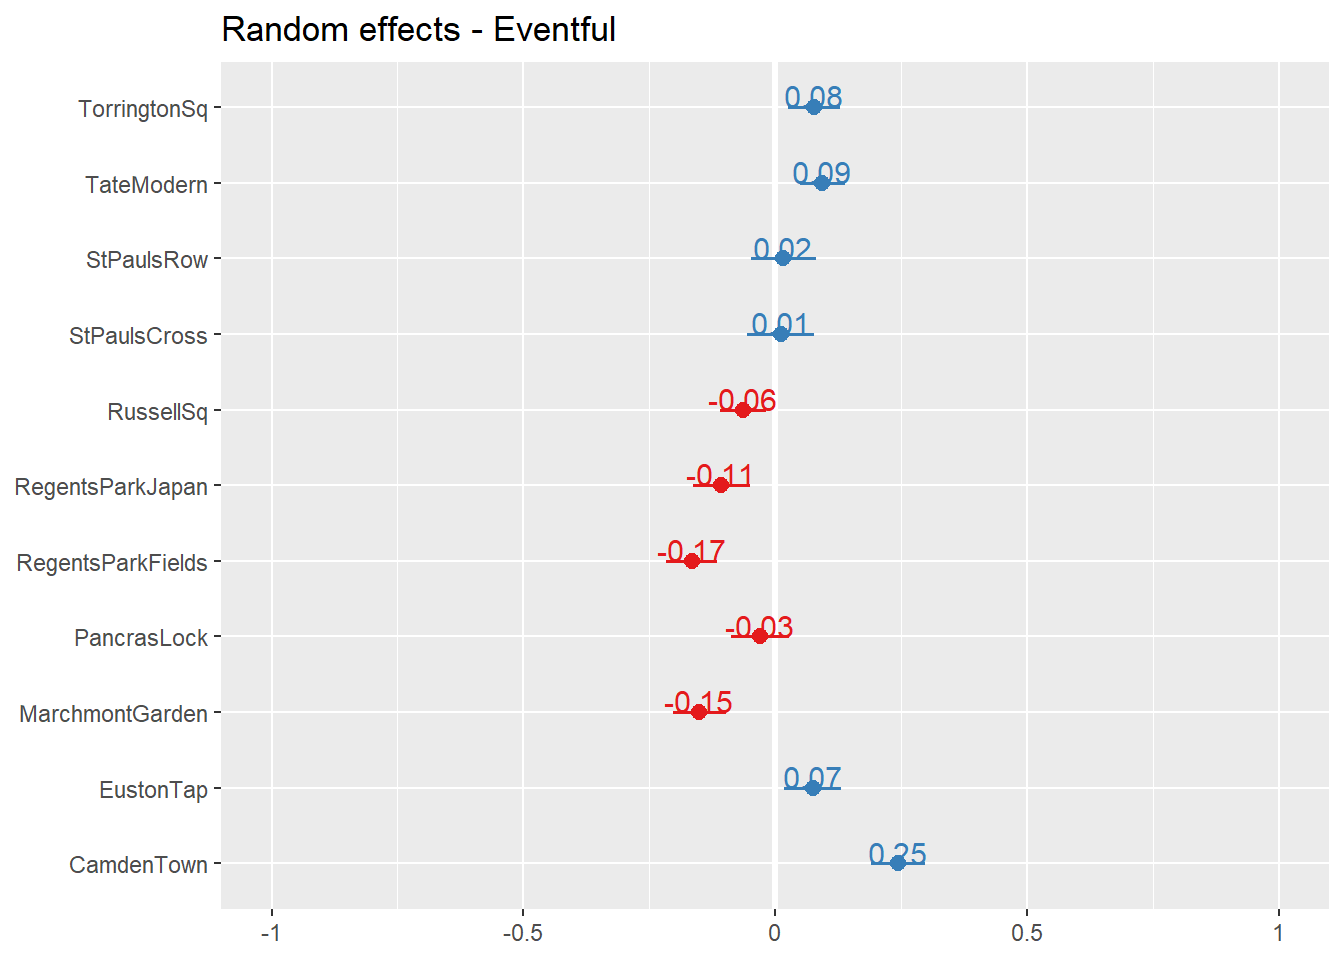
\includegraphics[width=\textwidth]{Figures/whoRandEvNew.png}
  \end{subfigure}
  \hfill
  \caption{The summary result demonstrated in the random-effects figures gives the average from the distribution of \gls{isopl} across locations.\label{fig:whoRand}}

\end{figure}


\subsubsection*{Occupation status}
According to our findings, occupation status, in particular `retirement' and to a lesser degree, gender (male) were important factors in the pattern of soundscape assessments. It is not clear why occupation (rather not say) demonstrates such a strong predictive relationship, either on its own or as an interaction term with \gls{who5}. A more detailed study or analysis will need to be performed to determine whether any other patterns around those who prefer not to state their occupation status can be found; it is possible that those who prefer not to say have some other characteristic which links them and somehow contributes to a change in their soundscape perception. We considered that `rather not say' may be viewed as the default response for some people, so if they were confused about the question or didn't fit in some other category, they would elect not to respond. However, this seems unlikely given that both `other' and `student' (possibly the most likely group to be unsure how to respond about their occupational status) were also options and did not reveal a strong relationship.

It is worthwhile to highlight that `retirement' factor could potentially be a proxy for age ($>65$) and gender (male). In order to further investigate the effect which the inclusion of occupational status had on the model building process, I re-ran the stepwise feature selection, this time without including occupation status in the initial model. This allowed me to determine whether other features (namely age and gender) would be finally selected and how they would interact within the model. The results of this process are given in \cref{tab:whoLMER2}.

\begin{table}
\centering
\caption{Linear mixed effects model resulting from the feature selection process when the initial model does not include occupational status. **$p<0.01$, *$p>0.05$  \label{tab:whoLMER2}}
\resizebox{\linewidth}{!}{%
\begin{tabular}{lccc|ccc} 
\toprule
 & \multicolumn{3}{c|}{\textbf{ISOPleasant}} & \multicolumn{3}{c}{\textbf{ISOEventful}} \\ 
\midrule
\textbf{Predictor} & \textbf{Estimates} & \textbf{Std. Est.} & \textbf{95\% CI} & \textbf{Estimates} & \textbf{Std. Est.} & \textbf{95\% CI} \\
WHO-5 & 0.001** & \textbf{0.03} & 0.01, 0.05 & - & - & - \\
Age & \textbf{0.001*} & \textbf{0.02} & 0.001, 0.04 & \textbf{-0.001**} & \textbf{-0.03} & -0.05, -0.01 \\
Gender (male) & - & - & - & \textbf{-0.04*} & \textbf{-0.04} & -0.07, -0.001 \\
Ethnicity & - & - & - & \textbf{-0.09**} & \textbf{-0.09} & 0.03, 0.14 \\ 
\midrule
\multicolumn{7}{l}{\textbf{Random Effects}} \\ 
\midrule
$\sigma^2$ & \multicolumn{3}{l|}{0.11} & \multicolumn{3}{l}{0.08} \\
$\tau_00$ & \multicolumn{3}{l|}{0.06$_{Location}$} & \multicolumn{3}{l}{0.01$_{Location}$} \\
ICC & \multicolumn{3}{l|}{0.34} & \multicolumn{3}{l}{0.14} \\
N & \multicolumn{3}{l|}{11} & \multicolumn{3}{l}{11} \\ 
\midrule
Observations & \multicolumn{3}{l|}{1134} & \multicolumn{3}{l}{1134} \\
Marginal/Conditional $R^2$ & \multicolumn{3}{l|}{0.009 / 0.345} & \multicolumn{3}{l}{0.023 / 0.165} \\
AIC & \multicolumn{3}{l|}{778.271} & \multicolumn{3}{l}{456.130} \\
\bottomrule
\end{tabular}
}
\end{table}

Age (\gls{isopl}: $\beta=0.02, p=0.05$; \gls{isoev}: $\beta=-0.03, p=0.01$) and gender (\gls{isoev}: $\beta=-0.04, p=0.05$) then came out as significant, as shown in \cref{tab:whoLMER2}. This would indicate that occupation status, particularly `retirement', represents a group of older male individuals. Even though incorporation of occupation into the model complicates the interpretation of the outcome, it results in a slightly better fitting model ($R^2_c$ for \gls{isopl} (0.354) and \gls{isoev} (0.181)) relative to 0.345 for \gls{isopl} and 0.165 for \gls{isoev} in the model without occupation status, which is why it is selected by the feature selection process. These findings are in line with previous research, suggesting significant differences among age groups in the soundscape of different acoustic environments \citep{Ren2016Soundscape,Yang2005Acoustic}. These findings imply that an increase in age leads to an increase in the positive appraisal of the soundscape pleasantness. This is supported by a study by \citet{Aydin2016Assessment} in which they found that soundscape pleasantness reported by young individuals was significantly lower than the other age groups.

Age could potentially highlight the contextual role of the acoustic environment. Past experiences, memories, and even traumas give a particular context to our perception and shape the soundscape, making individual perception highly diverse, depending on the content of experience/memory. While the increase in age can lead to appreciating different sound elements, lower age seems to be related to more arousing and vibrant sounds \citep{Yang2005Acoustic}.

Like age, gender was found to be associated with the soundscape eventfulness. Past works have also reported that there are gender-related discrepancies in soundscape \citep{Croome1977Noise,Yang2005Acoustic}. These differences may be an indication of different auditory processing across genders.

\section{Discussion}
The goal of this chapter was to determine to what extent secondary factors mediate soundscape perception, and to highlight which of these secondary factors are important to consider. 

As expected, the majority of the total variance in the perceptual ratings is explained by the location-level differences (e.g. overall sound level) which represent primary contributing factors to the acoustic environment (see \citet{McDermott2012Auditory}) and other non-acoustic factors. Approximately 3\% of the variance is then explained by the combination of personal factors, which represent secondary contributing factors as defined by McDermott. Although the variance explained by these secondary factors is small compared to the primary factors, they are still found to contribute significantly. 

\subsection{Incorporating personal factors}
Although, as \citet{Droumeva2021sound} points out, each individual brings their own cultural and subjective aspects of listening to the stage of urban sound, when attempting to characterise the soundscape of a space, it is not a particular individual's aspects we should be concerned with. That individual forms a part of the collective perception of the space. Their cultural and subjective (i.e. personal) aspects mitigate their perception, but this perception then forms only a single component of the collective perception. How then should we consider these personal factors? Surely there is no suggestion to disregard their influence and importance within the soundscape approach? In my view, there are two approaches:

\begin{enumerate}
  \item Incorporate these personal factors as demographic statistics of a location; or
  \item An agent-based approach where each individual likely to use the space is simulated and modelled with their personal factors to then be included in the collective perception.
\end{enumerate}

Let's look at how these two approaches would be implemented into the multilevel acoustics-based predictive model, such as those presented in \cref{ch:lockdown,ch:mlmann}.

\subsubsection{Approach 1}
In the first, the demographic breakdown of the space under investigation is estimated, either through a census or by the designers' desired use case. This demographic breakdown can then be compared to the results presented above \citep{Erfanian2021Psychological} to derive weighting factors which adjust the predicted soundscape assessment. For instance, the results suggest that retired persons perceive the soundscape as 0.01 points more pleasant than others. If the particular space under investigation has a large proportion of retired persons, say 65\% we could then apply an adjustment to the initial personal-factors-agnostic prediction to reflect this tendency. In this example, an initial location-level \gls{isopl} prediction of 0.36, with a 65\% retired population would be corrected by 0.0065 (0.65 x 0.01) for a final demographics-corrected \gls{isopl} prediction of 0.3665.

\subsubsection{Approach 2}
In the second approach, rather than performing an overall estimation of the demographics and soundscape perception distribution, individual responses (with their own probability estimation) are modelled. To illustrate this, let's assume that the modelling is performed for a 30 second section of audio; for a given day, we would then model a single response to each 30s audio, where the individual response, including adjustments for that individual's demographic features would be modelled. For any given individual, their likely demographic profile would be randomly drawn from the estimated demographic breakdown of the space -- i.e. if the space is expected to have 40\% men and 60\% women, there would be a 40\% chance that the individual modelled for a randomly selected 30s audio is a man and the appropriate feature coefficients would be used. The multiple individual responses are then summed to give the overall distribution of responses. Again, the general demographics of the space would need to be estimated in order to ensure that a reasonable distribution is used. This is a more direct implementation of the modelling presented in this chapter, directly using the models derived in this chapter, as opposed to deriving weighting factors as in approach 1.

\subsubsection{Strengths and limitations}
Without knowing the implementation of a final model (i.e. exactly how the input data is measured and fed through the system and the structure of the model), it is difficult to know which approach would be more or less difficult to implement. Assuming a system which generates a predicted distribution of responses for each 30s recording, it seems likely that both approaches would be equally simple to implement. However, approach 2 seems to offer one useful advantage; by applying the demographic corrections to each individual response prediction, it would be easier to appropriately include estimates for intra-correlated demographic characteristics. For instance, as illustrated in \cref{tab:whoLMER}, the \gls{isoev} has an interaction factor for psychological well-being (\gls{who5}) and gender (Male), so the proper breakdown both of the gender distribution and of the psychological well-being within the genders would be required. This seems much better suited to approach 2, where any individual's full personal profile could be created based on the factors which are likely to appear together (e.g. high psychological well-being and retired may be more prevalent in men than women and this would need to be reflected in the demographic statistics). 

On the other hand, again depending on the particular implementation of the final model, approach 1 would seem to be easier to exclude personal factors. As noted in \cref{sec:modelConstraints}, a robust model should allow us to define `optional' factors - ones which can be excluded from the model. Given their low impact and difficulty to estimate, personal and demographic factors will likely not always be available to include. If they are incorporated by applying weighting factors to the model predictions, then excluding them is as simple as not adding these weighting factors. 

\section{Conclusion}
In this chapter, we conducted a linear mixed-effects model to show the associations of psychological well-being and demographic factors with soundscape pleasantness and eventfulness. The findings indicate that psychological well-being is positively associated with pleasantness and negatively associated with eventfulness in males and individuals that did not report their occupations. We further demonstrated that the occupational status, in particular retirement as a proxy of age and gender, was related to the perceptions of pleasantness and eventfulness. In total, these personal factors were shown to account for 1.4\% of the variance for pleasantness and 3.9\% of the variance for eventfulness. These results confirm, to some degree, the results presented in \cref{ch:mlmann}, where gender was not found to be a significant predictor of annoyance. If we take annoyance to be the inverse of pleasantness, then both analyses reveal there is not a statistically significant relationship between gender and the perception of pleasantness/annoyance. However, the results of this chapter do demonstrate that gender, both on its own and when paired with psychological well-being has a significant impact on a person's perception of the eventfulness of a soundscape. This further demonstrates the limitations of previous noise control studies which, at most, aimed to investigate only the annoyance dimension. It is important to ensure that we are not disregarding the secondary dimension of soundscape perception. 

I then offer a series of proposals for how these personal factors can be included in a predictive modelling framework to enable soundscape predictions to account for differences in demographic patterns. At some point, it seems necessary that a truly holistic approach to soundscape design will need to account for these differences, particularly as we begin to make better comparisons across countries and cultures. However, given the level of uncertainty still present in soundscape predictions and the relatively low explanatory demonstrated for these demographic features, at this point it does not appear that further exploring personal factors in a predictive modelling context is the most necessary step. Other, more impactful features such as including sound sources and visual features, are more important for creating accurate and useful predictive models. That said, the inclusion of psychological well-being (as measured by \gls{who5}) does provide new empirical grounds for research to explore the influence of one's psychological state on their perception and experience of complex sound environments.
